\chapter{Веб-платформа как открытая, кроссплатформенная среда для создания информационных систем}

Веб-платформа — набор технологий, разработанных в виде открытых стандартов, такими организациями как W3C, WHATWG, IETF, ECMA, и т.д. Веб-платформа включает в себя компьютерные языки и API-интерфейсы. Этот набор технологий описывается в стандартах HTML, CSS, ECMAScript, SVG, WebAssembly, MathML, HTTP, WOFF, и т.д.

Существует множество реализаций спецификаций веб-платформы, в их число входят браузеры — Chrome, Safari, FireFox, Edge, и др., серверные среды — Node.js, Deno, Bun, и др. Каждая из реализаций имплементирует лишь некоторую часть из всех спецификаций.

В настоящее время, существует проект Web Platform Tests (WPT), который представляет собой набор тестов для спецификаций веб-платформы, проверяющих соответствие реализаций веб-стандартов спецификациям. WPT поддерживается консорциумом W3C, а также сообществом разработчиков браузеров. Цель проекта — обеспечить более высокую степень совместимости между различными реализациями и улучшить качество веб-платформы в целом. Результаты тестирования WTP используются для проверки соответствия реализаций стандартам веб-платформы, а также для обеспечения совместимости веб-приложений на различных платформах и устройствах, результаты тестирования показаны на рисунке \ref{fig:web-platform-tests}.

\begin{figure}[H]
\begin{center}
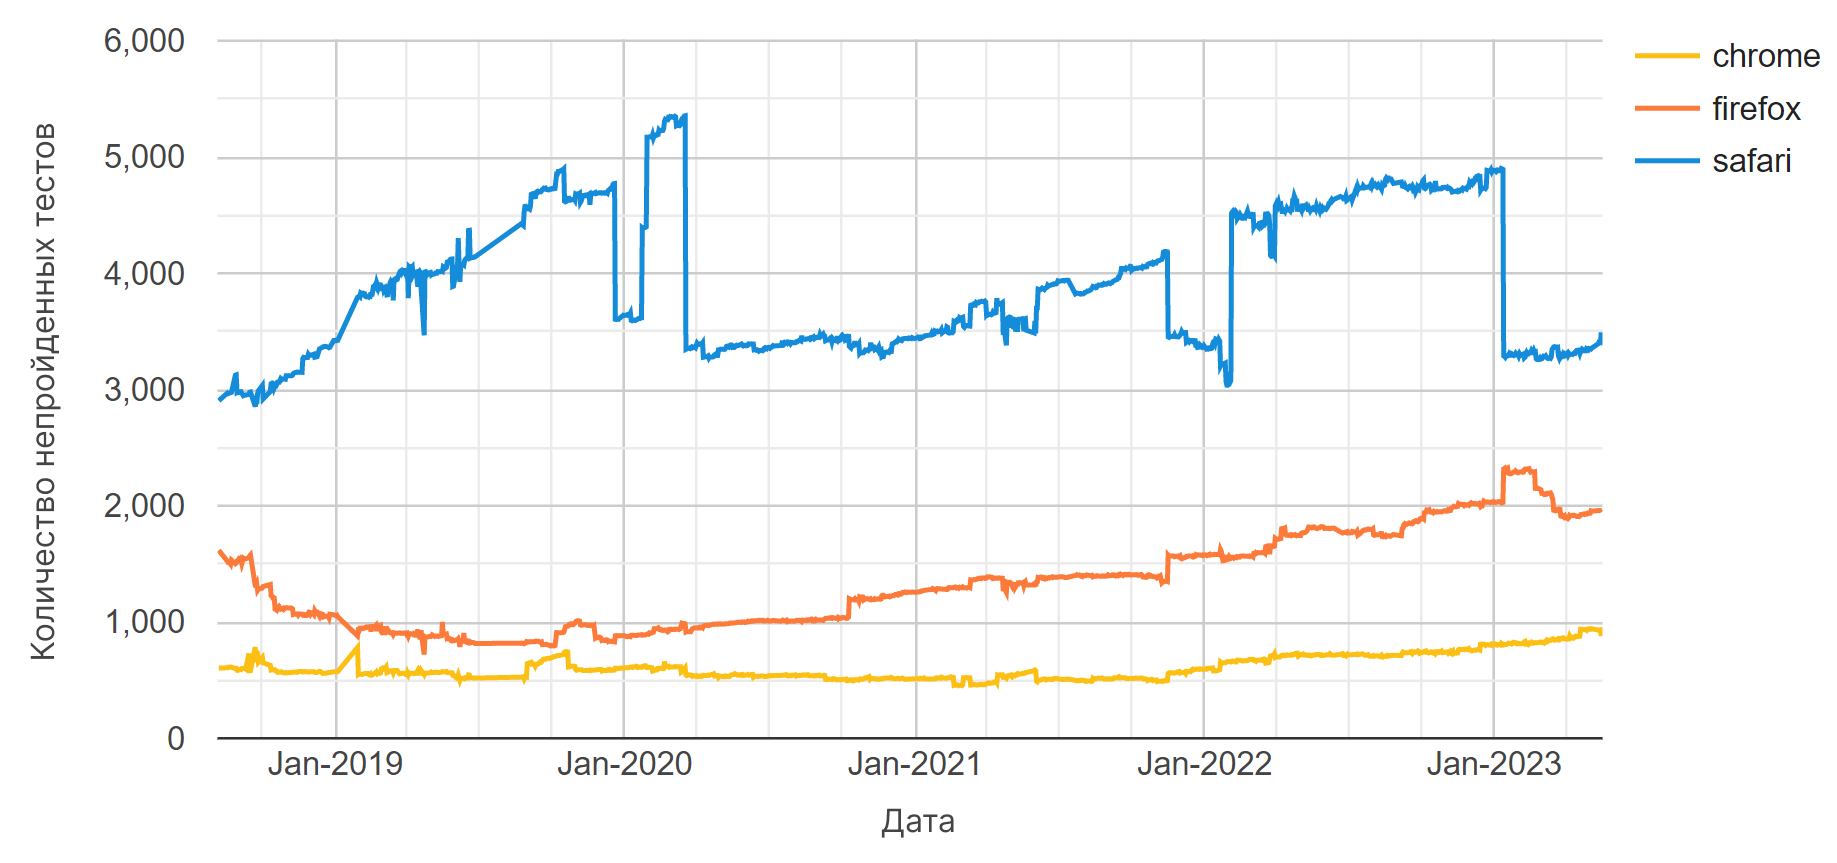
\includegraphics[width=1.0\hsize]{fig/web-platform-tests.png}\\[2mm]
\caption{Результаты Web Platform Tests}\label{fig:web-platform-tests}
\end{center}
\end{figure}

\section{Подход прогрессивных веб-приложений (PWA) и новые API-интерфейсы веб-платформы для реализации функционала платформо-зависимых приложений}

Progressive Web Apps (PWA) — это веб-приложение, созданное с использованием веб-технологий, но обеспечивающее взаимодействие с пользователем, аналогично платформо-зависимым приложениям \cite{pwaJason}. Принцип работы различных видов приложений показан на рисунке \ref{fig:pwa-environment}.

\begin{figure}[H]
\begin{center}
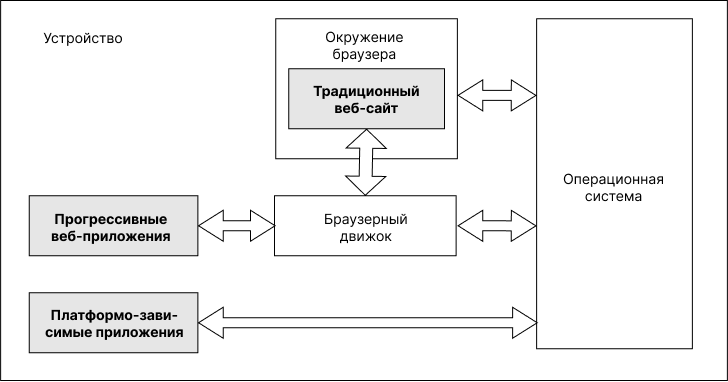
\includegraphics[width=1.0\hsize]{fig/pwa-environment.png}\\[2mm]
\caption{Принцип работы различных видов приложений}\label{fig:pwa-environment}
\end{center}
\end{figure}

Традиционные веб-сайты имеют некоторые преимущества по сравнению с платформо-зависимыми приложениями:

\begin{enumerate} 
  \item Единая кодовая база. Поскольку Интернет является кроссплатформенным, веб-сайт может работать на разных операционных системах и устройствах.
  
  \item Распространение через Интернет. Веб-сайты индексируются поисковыми системами, ими можно поделиться и получать к ним доступ только с помощью URL-адресов.
\end{enumerate}

Прогрессивные веб-приложения сочетают в себе подходы традиционных веб-сайтов и платформо-зависимых приложений, обладая следующими преимуществами:

\begin{enumerate} 
  \item PWA разрабатываются с использованием стандартных технологий веб-платформы, поэтому являются кроссплатформенными.
  
  \item Доступ к PWA можно получить из Интернета, как к обычному веб-сайту.

  \item PWA можно установить в операционную систему. Установленное прогрессивное веб-приложение запускается в отдельном окне вместо окружения браузера, их можно запустить с главного экрана или панели задач.

  \item PWA может работать в фоновом и автономном режиме.

  \item PWA может в фоновом режиме обрабатывать push-сообщения с сервера и отображать уведомления с помощью нативной системы уведомлений ОС.

  \item PWA может быть целью для отправки информации из других приложений или отправлять информацию другим установленным приложениям через общий канал.

  \item PWA можно регистрировать в качестве приложения по умолчанию для обработки различных типов файлов.
\end{enumerate}

\subsection{Манифест веб-приложения}

Манифест веб-приложения — это JSON файл, который сообщает браузеру о прогрессивном веб-приложении и о том, как оно должно вести себя при инсталляции в операционную систему. Файл манифеста традиционно называется «manifest», согласно спецификации, расширение файла должно быть «.webmanifest» \cite{webmanifest}.

Ключевые свойства веб-манифеста:

\begin{enumerate} 
  \item name/short\_name — если указаны оба, то short\_name используется на главном экране операционной системы, в панели запуска или других интерфейсах ОС, name используется при установке приложения. Некоторые браузеры добавляют «short\_name» к тому, что указано в теге \verb|<title>| HTML-документа, этот заголовок отображается на различных поверхностях переключения окон.
  
  \item id — позволяет явно определить идентификатор, используемый для веб-приложения.

  \item start\_url — сообщает браузеру о том, какая страница должна быть открыта, когда пользователь запустит приложение с домашнего экрана.

  \item icons — массив объектов изображения. Каждый объект должен включать в себя свойства src, sizes и type изображения. Значки используются на главном экране, панели запуска приложений, при переключении между приложениями и т.д.

  \item display — определяет окружение, в котором будет запускать прогрессивное веб-приложение. «fullscreen» — запустит веб-приложение без какого-либо стороннего пользовательского интерфейса, предоставив всю доступную область отображения. «standalone» — запустит веб-приложение в отдельном окне, вид интерфейса окна приложения будет зависеть от операционной системы. «minimal-ui» — предоставляет пользователю минимальный набор элементов пользовательского интерфейса для управления навигацией (например кнопку назад). «browser» — запустит веб-приложение в традиционном окружении браузера.

  \item theme\_color — определяет цвет окна веб-приложения, также может отразиться в предварительном просмотреть приложения в переключателях задач.

  \item background\_color — определяет цвет фона во время запуска и установки веб-приложения.

  \item screenshots — массив объектов изображения, представляющих веб-приложение в различных сценариях использования.
\end{enumerate}

\subsection{Способы установки прогрессивного веб-приложения в операционную систему}

Наличие нескольких каналов распространения приложения — мощный способ охватить большое число пользователей. Прогрессивное веб-приложение может быть установлено следующими способами:

\begin{enumerate} 
  \item Установка через интерфейс браузера. Пользователь может установить PWA, открыв веб-приложение в браузере и выбрав опцию «Установить» в контекстном меню браузера. Этот способ доступен в большинстве современных браузеров, таких как Google Chrome, Mozilla Firefox, Microsoft Edge и Safari. Также некоторые браузеры сами предложат установить веб-приложение в операционную систему, при первом заходе пользователя (рисунок \ref{fig:install-browser}).

\begin{figure}[H]
\begin{center}
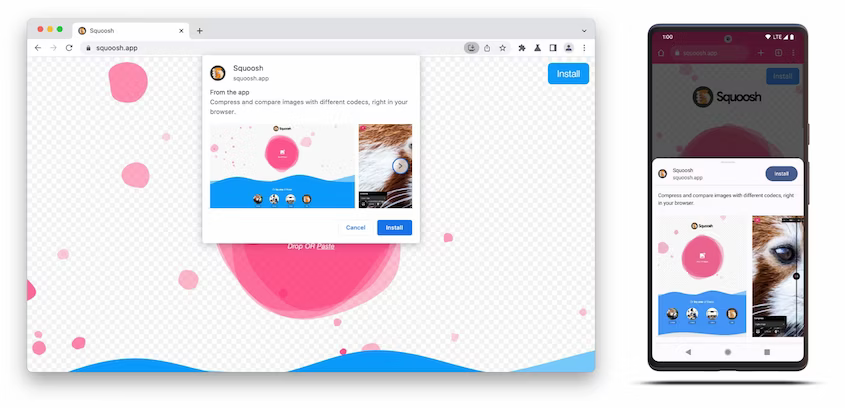
\includegraphics[width=1.0\hsize]{fig/install-browser.png}\\[2mm]
\caption{Предложение установить прогрессивного веб-приложения через интерфейс браузера}\label{fig:install-browser}
\end{center}
\end{figure}
  
  \item Установка через интерфейс веб-приложения. Помимо возможностей установки, предоставляемых браузером, можно создать собственный процесс установки непосредственно в приложении (рисунок \ref{fig:install-promt}). Браузерный API предоставляет событие «beforeinstallprompt», которое вызывается, когда пользователь может установить PWA в операционную систему, с помощью его обработки, разработчики могут реализовать свою логику продвижения установки веб-приложения.

\begin{figure}[H]
\begin{center}
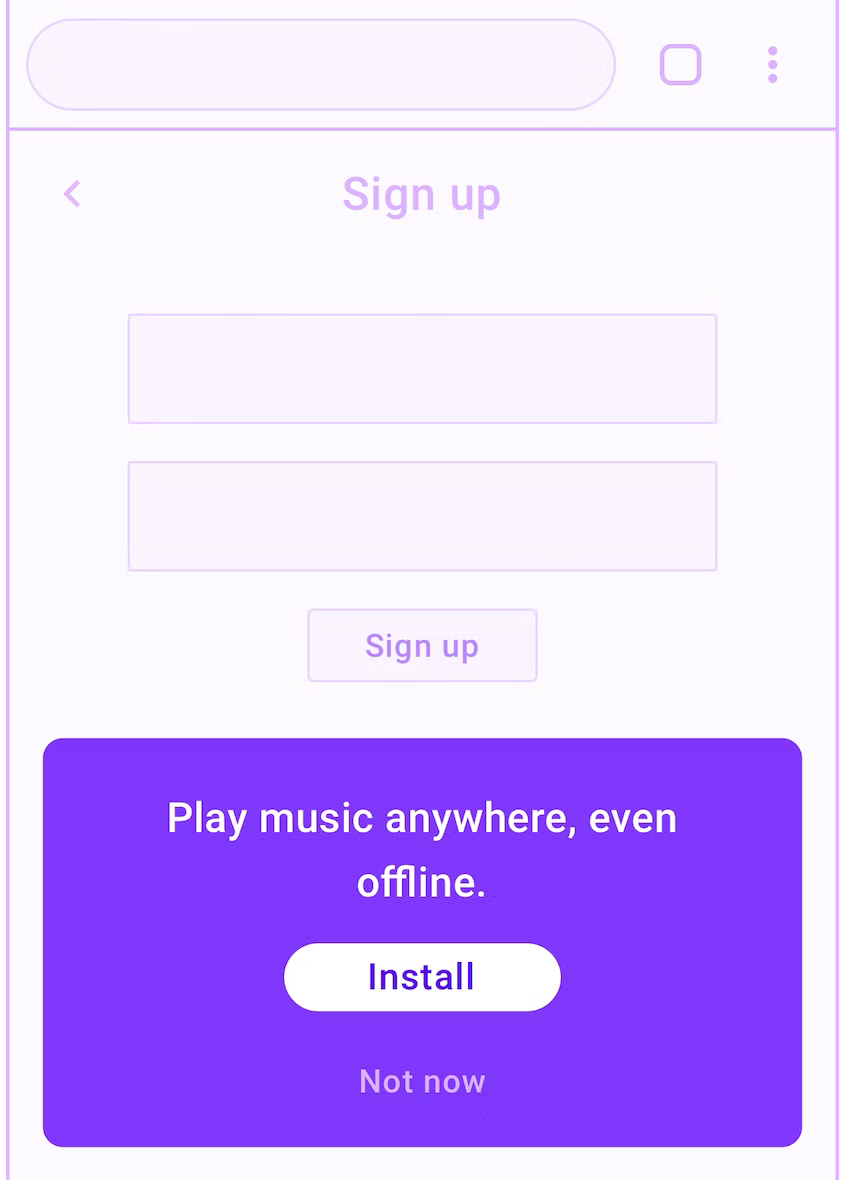
\includegraphics[width=0.6\hsize]{fig/install-promt.png}\\[2mm]
\caption{Пример продвижения установки прогрессивного веб-приложения, реализованный разработчиком}\label{fig:install-promt}
\end{center}
\end{figure}

  \item Установка через магазин приложений. Некоторые операционные системы, такие как Android, Windows, iOS, имеют магазины приложений, любое прогрессивное веб-приложение может быть собрано под конкретную операционную систему, для распространения через магазин приложений. Так ОС Android имеет технологию Trusted Web Activity, которая обеспечивает отображение прогрессивных веб-приложений в полноэкранном режиме и гарантирует, что контейнеры Trusted Web Activity будут в той же степени совместимы с функциями и API веб-платформы, что и используемый браузер, это позволяет сильно уменьшить размер веб-приложения, загружаемого в магазин. PWABuilder — инструмент с открытым исходным кодом, который дает возможность автоматизировать сборку прогрессивных веб-приложений под конкретные операционные системы.
\end{enumerate}

\subsection{Service Workers. Кэширование ресурсов веб-приложения. Сетевые стратегии, автономный режим работы. Стратегии обновления веб-приложения}

Service Workers являются фундаментальной частью прогрессивных веб-приложения. Они обеспечивают загрузку веб-приложения независимо от состояния сети, push-уведомления с сервера и другие возможности.

Service Worker — управляемый событиями worker, который может перехватывать и изменять запросы навигации и ресурсов, что позволяет использовать различные стратегии кэширования и обновления ресурсов \cite{serviceWorker}.

Service Worker запускается в отдельном контексте и потоке, не имеет доступа к DOM. Из соображений безопасности, Service Worker API работает только через HTTPS соединение.

Для кэширования ресурсов, можно использовать API хранилища Service Worker. Этот API работает аналогично стандартному кэшу браузера. Чтобы реализовать простейшее кэширование статических ресурсов, нужно добавить обработку события «install», внутри обработчика необходимо открыть кэш и добавить в него ресурсы, которые нужно кэшировать (листинг \ref{ls:simple-cache}).

\begin{lstlisting}[caption={Простейшее кэширование статических ресурсов}, label={ls:simple-cache}]
self.addEventListener('install', function(event) {
  event.waitUntil(
    caches.open('my-cache').then(function(cache) {
      return cache.addAll([
        '/',
        '/index.html',
        '/styles.css',
        '/script.js',
        '/image.jpg'
      ]);
    })
  );
});
\end{lstlisting}

Сетевые стратегии определяют, как Service Worker будет обрабатывать запросы к серверу. Существуют различные стратегии, такие как «cache-first», «network-first», «cache-only», «network-only» и другие. Каждая стратегия определяет, как Service Worker будет использовать кэш и сеть для получения ресурсов.

Стратегия «network-only» — при использовании этой стратегии Service Worker делает запрос к серверу и возвращает ответ. Если запрос не удался, то Service Worker возвращает ошибку (рисунок \ref{fig:network-only}). Эта стратегия подходит для ресурсов, которые должны быть доступны только при наличии подключения к сети.

\begin{figure}[H]
\begin{center}
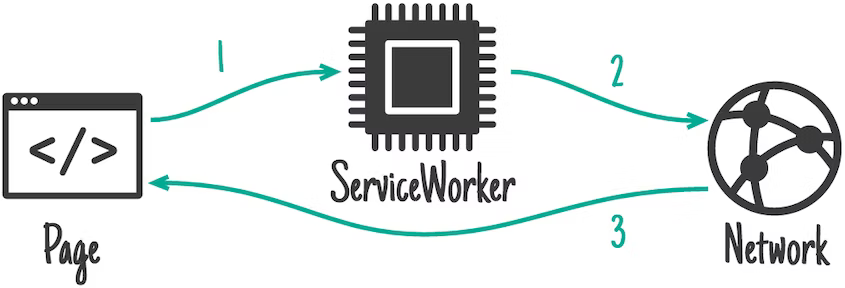
\includegraphics[width=1.0\hsize]{fig/net-only.png}\\[2mm]
\caption{Принцип работы стратегии кэширования «network-only»}\label{fig:network-only}
\end{center}
\end{figure}

Стратегия «cache-only» — при использовании этой стратегии Service Worker проверяет наличие кэшированного ресурса и, если он есть, возвращает его. Если кэш пустой, то Service Worker не делает запрос к серверу и возвращает ошибку (рисунок \ref{fig:cache-only}). Эта стратегия подходит для ресурсов, которые должны быть доступны только в автономном режиме.

\begin{figure}[H]
\begin{center}
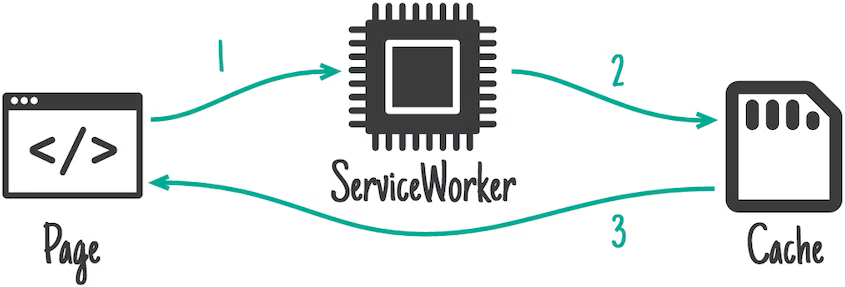
\includegraphics[width=1.0\hsize]{fig/cache-only.png}\\[2mm]
\caption{Принцип работы стратегии кэширования «cache-only»}\label{fig:cache-only}
\end{center}
\end{figure}

Стратегия «network-first» — при использовании этой стратегии Service Worker сначала делает запрос к серверу и возвращает ответ. Если запрос не удался, то Service Worker проверяет наличие кэшированного ресурса и, если он есть, возвращает его (рисунок \ref{fig:network-first}). Эта стратегия подходит для ресурсов, которые меняются часто, например, новостей или социальных сетей.

\begin{figure}[H]
\begin{center}
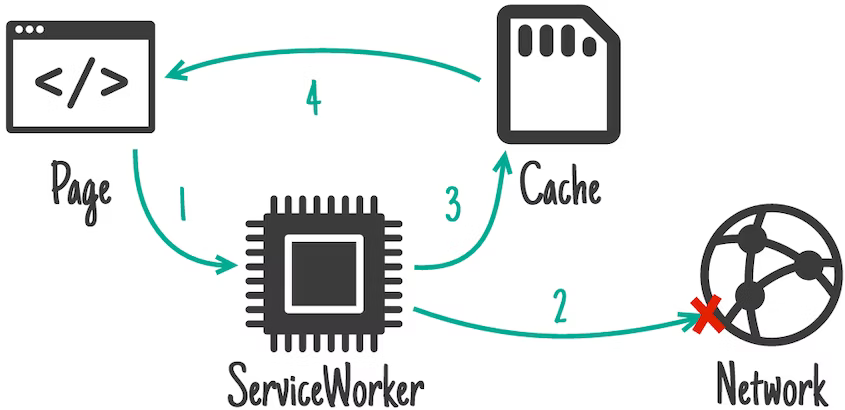
\includegraphics[width=1.0\hsize]{fig/net-first.png}\\[2mm]
\caption{Принцип работы стратегии кэширования «network-first»}\label{fig:network-first}
\end{center}
\end{figure}

Стратегия «cache-first» — при использовании этой стратегии Service Worker сначала проверяет наличие кэшированного ресурса и, если он есть, возвращает его. Если кэш пустой, то Service Worker делает запрос к серверу и возвращает ответ, после чего помещает его в кэш (рисунок \ref{fig:cache-first}). Это отличная стратегия для применения ко всем статическим активам (таким как CSS, JavaScript, изображения и шрифты), особенно к тем, которые имеют хэш-версию. Он предлагает повышение скорости для неизменяемых активов, обходя любые проверки свежести контента с сервером, который может запускать кеш HTTP. Что еще более важно, любые кэшированные ресурсы будут доступны в автономном режиме.

\begin{figure}[H]
\begin{center}
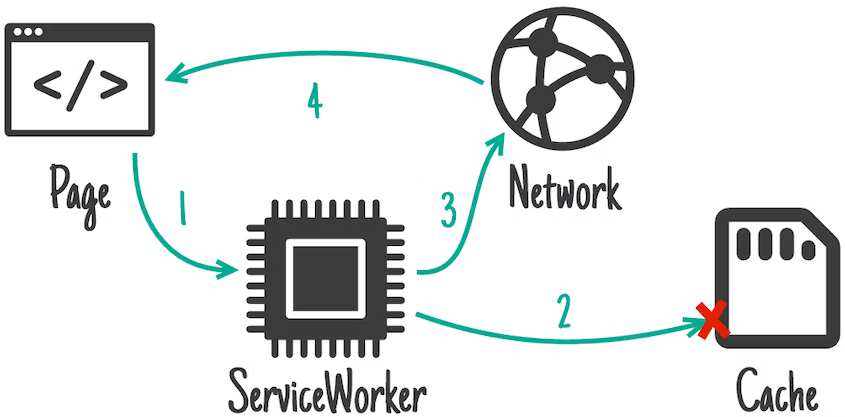
\includegraphics[width=1.0\hsize]{fig/cache-first.png}\\[2mm]
\caption{Принцип работы стратегии кэширования «cache-first»}\label{fig:cache-first}
\end{center}
\end{figure}

Таким образом, при помощи комбинирования стратегий «cache-first» и «network-first», можно разрабатывать веб-приложения, функционирующие без доступа к сети. Для этого необходимо кэшировать все статически ресурсы по стратегии «cache-first», а запросы к серверному API при помощи «network-first», тогда, при запуске приложения в автономном режиме, пользователь сможет выполнять навигацию по приложению и просматривать ту информацию, которая была доступна ранее.

За счет того, что в названии каждого статического ресурса используется специальный хэш, при развертывании новой версии веб-приложения, хэш тех ресурсов, которые были обновлены меняется, таким образом, браузер узнает о том, что появилась новая версия веб-приложения. В этом случае необходимо обновить кэшированные ресурсы, чтобы пользователи могли использовать последнюю версию приложения. Существует две основные стратегии для обновления ресурсов веб-приложения:

\begin{enumerate} 
  \item Автоматическое обновление (auto-update)  — при использовании этой стратегии Service Worker автоматически обновляет кэшированные ресурсы, когда меняется их хэш. Это означает, что пользователи будут использовать последнюю версию приложения без необходимости обновления страницы вручную. Автоматическое обновление может быть удобным для пользователей, которые хотят использовать последнюю версию приложения без необходимости обновления страницы вручную. Однако, это может привести к потере данных, если обновление произойдет во время работы пользователя с приложением.
  
  \item Оповещение пользователя (promt-update)  — при использовании этой стратегии, разработчик реализует оповещение о том, что появилась новая версия приложения, и предлагает обновить страницу (рисунок \ref{fig:promt-uptate}). Это позволяет пользователям сохранить свои данные и решить, когда им обновить страницу. Однако, это может привести к тому, что пользователи не обновят страницу вовремя и будут продолжать использовать устаревшую версию приложения.  
\end{enumerate}

\begin{figure}[H]
\begin{center}
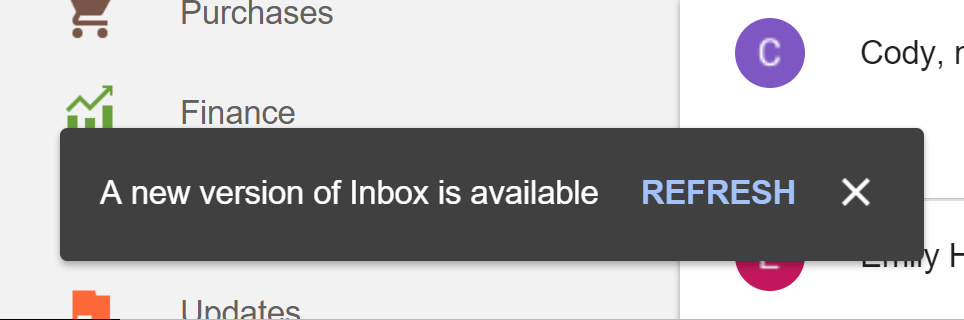
\includegraphics[width=1.0\hsize]{fig/service-worker-promt-uptate.png}\\[2mm]
\caption{Пример оповещения пользователя о том, что доступно обновление веб-приложения}\label{fig:promt-uptate}
\end{center}
\end{figure}

\section{Современные методы и подходы для оптимизации и ускорения веб-приложений}

С увеличением функционала и сложности веб-приложений, оптимизация и ускорение веб-приложений стали ключевыми факторами для обеспечения положительного пользовательского опыта.

Оптимизация производительности веб-приложений является важным аспектом разработки, поскольку она напрямую влияет на удовлетворенность пользователей, конверсию и, в конечном итоге, успех проекта. Быстрые и отзывчивые веб-приложения улучшают пользовательский опыт, уменьшают время загрузки страниц и снижают отказы от использования приложения.

Применение современных методов и подходов оптимизации производительности веб-приложений позволяет достичь следующих преимуществ:

\begin{enumerate} 
  \item Улучшение пользовательского опыта. Быстрые и отзывчивые веб-приложения обеспечивают более комфортное взаимодействие, что способствует удержанию и привлечению новых пользователей.
  
  \item Повышение конверсии. Оптимизированные веб-приложения увеличивают вероятность выполнения целевых действий пользователями, таких как покупка товаров или услуг.

  \item Снижение нагрузки на сервер. Оптимизация производительности веб-приложений может снизить нагрузку на сервер, что в свою очередь снижает затраты на обслуживание и масштабирование инфраструктуры.

  \item Улучшение позиций в поисковых системах. Быстрые и оптимизированные веб-приложения получают более высокие оценки от поисковых систем, что способствует повышению трафика.
\end{enumerate}

\subsection{Оптимизация на стороне сервера. Использование алгоритмов сжатия, HTTP/3 и Content Delivery Network (CDN)}

Серверная оптимизация является важным компонентом улучшения производительности веб-приложений. Серверная оптимизация влияет на ряд ключевых метрик, которые напрямую связаны с производительностью веб-приложений и пользовательским опытом. При применении серверной оптимизации улучшаются следующие метрики:

\begin{enumerate} 
  \item Время отклика сервера (Time to First Byte, TTFB). Это время, затраченное на получение первого байта данных от сервер после отправки запроса.
  
  \item Пропускная способность (Throughput). Это количество данных, которое сервер может обрабатывать и передавать за определенный промежуток времени.

  \item Количество одновременных соединений (Concurrency). Это количество одновременных запросов, которые сервер может обрабатывать.

  \item Устойчивость к потере пакетов (Packet Resilience). Оптимизация сервера, особенно с использованием протокола HTTP/3, может улучшить устойчивость к потере пакетов, снижает вероятность задержек и повторных передач данных.

  \item Время загрузки страницы (Page Load Time). Это время, необходимое для полной загрузки и отображения контента на веб-странице.
\end{enumerate}

Алгоритмы сжатия, такие как Gzip и Brotli, позволяют сократить объем передаваемых данных между сервером и клиентом, уменьшая время загрузки страниц и улучшая пользовательский опыт. Сжатие ресурсов, таких как HTML, CSS и JavaScript может значительно уменьшить их размер, что приводит к быстрому отображению контента на стороне пользователя \cite{compression}.

GNU Zip (gzip) является стандартным методом сжатия в UNIX-системах, который широко используется в веб-разработке. Является встроенным методом сжатия в веб-сервер NGINX.

Brotli — более новый алгоритм сжатия данных с открытым исходным кодом, разработанный внутри компании Google, является более эффективной альтернативой gzip.

Существует два основных метода применения алгоритмов сжатия:

\begin{enumerate} 
  \item Предварительное сжатие статических ресурсов. Такие ресурсы как HTML, CSS, JavaScript и изображение, могут быть предварительно сжаты при сборке веб-приложения, что может значительно уменьшить размер файлов и ускорить их передачу с сервера на клиент. Данный метод следует применять по умолчанию.
  
  \item Сжатие ресурсов в момент запроса. Это может быть полезно для динамически генерируемых страниц, которые не могут быть сжаты предварительно. Сжатие в момент запроса может ухудшить производительность сервера, поэтому его следует использовать с осторожностью.
\end{enumerate}

Для уменьшения задержек при передачи данных, следует использовать последнюю версию протокола передачи гипертекста. HTTP/3 – это новая версия протокола передачи гипертекста, основанный на протоколе QUIC, основным улучшением в сравнении с HTTP/2 и HTTP/1.1 является уменьшение задержки при установлении соединения, улучшенное мультиплексирование и повышенная устойчивость к потере пакетов \cite{webserverhttp3}.

Согласно статистике сервиса «Can I Use», на сегодняшний день протокол HTTP/3 полностью поддерживается у 73.66\% клиентов и еще частично поддерживается 19.06\%, что в совокупности составляет 92.71\% \cite{caniusehttp3}.

Исходя из статистики и получаемых преимуществ, уже сейчас стоит использовать протокол HTTP/3, как прогрессивное улучшение. Если браузер клиента не поддерживает HTTP/3, то сервер автоматически переключится на HTTP/2 или HTTP/1.1, в зависимости от возможностей браузера Это означает, что веб-сайт будет доступен для всех пользователей, независимо от того, поддерживает ли их браузер HTTP/3 или нет.

Использование подхода Content Delivery Network (CDN) может значительно ускорить доставку ресурсов от сервера к клиенту. CDN — это сеть распределенных серверов, которые хранят копии статических ресурсов веб-сайта и доставляют их пользователям, исходя из ближайшего географического местоположения.

Данный подход ускоряет загрузку страницы, за счет того, что минимизирует расстояние между клиентов и сервером. Помимо этого, улучшается доступность веб-сайта, поскольку если один из серверов в сети CDN недоступен, клиент сможет получить контент через другой сервер распределенной сети. Также суммарная нагрузка на систему распределяется между всеми серверами в сети.

\subsection{Управление загрузкой ресурсов в веб-приложении. Встряхивание дерева зависимостей. Lazy-Loading Routes и Fetch Priority API}

Управление загрузкой ресурсов в веб-приложении является ключевым фактором для обеспечения высокой производительности и оптимального пользовательского опыта.

Встряхивание дерева зависимостей (Tree-shaking) — техника позволяющая уменьшить размер финального пакета (bundle) веб-приложения, исключая неиспользуемый код из зависимостей. Современные сборщики, такие как Vite и Webpack, автоматически выполняют встряхивание дерева при сборке веб-приложения, что позволяет сократить объем загружаемых ресурсов и ускорить время загрузки.

Ленивая загрузка маршрутов (Lazy-Loading Routes) — отложенная загрузка компонентов веб-приложения до тех пор, пока они не понадобятся клиенту. Это позволяет разделить кодовую базу веб-приложения на маленькие части (chunks) и загружать их по мере необходимости, что сокращает время начальной загрузки и улучшает производительность. Библиотеки реазилующие маршрутизацию на стороне клиента, как правило, предоставляют встроенные механизмы для реализации ленивой загрузки маршрутов.

Когда браузер анализирует веб-страницу и начинает обнаруживать и загружать такие ресурсы, как изображения, скрипты и стили, он назначает им приоритет, пытаясь загрузить ресурсы в оптимальном порядке. Эти приоритеты могут зависеть от типа ресурса и его места в документе. Например, изображение в видимой области просмотра, может иметь «high» приоритет, в то время, как блокирующие рендеринг стили могут иметь приоритет «very high». Новый HTML-атрибут «fetchpriority» позволяет разработчикам вручную управлять приоритезацией загрузки ресурсов.

Приоритет Fetch API (Fetch Priority API) — параметр, определяющий относительный приоритет конкретного ресурса. Указать приоритет можно в HTML разметке, при помощи атрибута «fetchpriority», а также с помощью свойства «priority» в Fetch API.

Атрибут «fetchpriority» может быть использован с тегами link, img и script. Атрибут принимает одно из трех значений:

\begin{enumerate} 
  \item high — ресурс имеет высокий приоритет, браузер будет отдавать приоритет ему до тех пор, пока эвристика браузера не препятствует этому.
  
  \item low — ресурс имеет низкие приоритет, браузер загрузит его в последнюю очередь, если это позволяет эвристика.

  \item auto — значение по умолчанию, браузер сам определит соответствующий приоритет.
\end{enumerate}

Важно отметить, что параметр устанавливает относительный приоритет, то есть он повышает или понижает приоритет по умолчанию на соответствующую величину, а не явно устанавливает приоритет загрузки.

\subsection{Методы оптимизации загрузки и рендеринга веб-шрифтов}

Веб-шрифты являются важным элементом многих веб-сайтов, однако, неправильное использование и загрузка веб-шрифтов может привести к снижению производительности и ухудшению пользовательского опыта.

Существует несколько проблем, связанных с веб-шрифтами:

\begin{enumerate} 
  \item Отложенный рендеринг текста. Если веб-шрифт не загружен на устройство клиента, браузеры обычно задерживают рендеринг текста. Во многих случаях это приводит к задержке метрики First Contenful Paint (FCP), а также Largest Contenful Paint (LCP).
  
  \item Сдвиг макета. Практика замены шрифтов может привести к сдвигу макете, тем самым повлияв на метрику Cumulative Layout Shift (CLS). Эти изменения макета происходят, когда веб-шрифт и его резервный шрифт занимают разное количество места на странице.
\end{enumerate}

Шрифты, как правило, являются важными ресурсами, так как без них пользователь не сможет просматривать содержимое страницы. Таким образом, рекомендации по загрузке шрифтов обычно направлены на то, чтобы шрифты загружались как можно раньше, это может быть реализовано с помощью HTML-атрибутов «fetchpriority» и «preload».

Из современных шрифтов WOFF2 является самым эффективным, имеет широкую поддержку браузеров и предлагает лучшее сжатие. Поскольку он использует алгоритм сжатия Brotli, WOFF2 весит в среднем на 30\% меньше, чем WOFF, что приводит к загрузке меньшего количества данных и, следовательно, более высокой производительности. Учитывая браузерную поддержку, рекомендуется использовать  формат WOFF2 по умолчанию.

Файлы шрифтов содержат большое количество глифов для различных символов, которые они поддерживают. На практике, размер веб-шрифта Google Fonts обычно составляет 30-40 КБ, а если учесть, что зачастую используются разные начертания шрифта, общий вес всех шрифтов может составлять 200-300 КБ.

Как правильно, на сайте используется ограниченный алфавит, значительно меньше того, что содержит шрифт, исходя из этого, можно выделить определенное подмножество из шрифта, для уменьшения его размера.

Дескриптор «unicode-range» в \verb|@font-face| объявлении сообщает браузеру, для каких символов можно использовать шрифт (листинг \ref{ls:unicode-range}).

\begin{lstlisting}[caption={Пример определения unicode диапозона}, label={ls:unicode-range}]
@font-face {
    font-family: "Open Sans";
    src: url("/fonts/OpenSans-Regular-webfont.woff2") format("woff2");
    unicode-range: U+0025-00FF;
}
\end{lstlisting}

Файл шрифта будет загружен, если страница содержит один или несколько символов, соответствующих диапазону Unicode. Например, вместо предоставления полного набора символов, можно создать отдельные подмножества шрифтов для символов латиницы и кириллицы (листинг \ref{ls:font-subsets}). Удаление неиспользуемых глифов может значительно уменьшить размер шрифта, вплоть до 10-кратного уменьшения размера.

\begin{lstlisting}[caption={Пример создания нескольких подмножеств шрифта}, label={ls:font-subsets}]
/* devanagari */
@font-face {
  font-family: 'Poppins';
  font-style: normal;
  font-weight: 400;
  font-display: swap;
  src: url(https://fonts.gstatic.com/s/poppins/v20/pxiEyp8kv8JHgFVrJJbecnFHGPezSQ.woff2) format('woff2');
  unicode-range: U+0900-097F, U+1CD0-1CF6, U+1CF8-1CF9, U+200C-200D, U+20A8, U+20B9, U+25CC, U+A830-A839, U+A8E0-A8FB;
}
/* latin-ext */
@font-face {
  font-family: 'Poppins';
  font-style: normal;
  font-weight: 400;
  font-display: swap;
  src: url(https://fonts.gstatic.com/s/poppins/v20/pxiEyp8kv8JHgFVrJJnecnFHGPezSQ.woff2) format('woff2');
  unicode-range: U+0100-024F, U+0259, U+1E00-1EFF, U+2020, U+20A0-20AB, U+20AD-20CF, U+2113, U+2C60-2C7F, U+A720-A7FF;
}
\end{lstlisting}

\subsection{Оптимизация загрузки изображений. Выбор правильного формата. Замена анимированных GIF на видео. Адаптивная и отложенная загрузка}

Изображения являются одними из самых популярных ресурсов на веб-страницах, и их оптимизация играет важную роль в улучшении производительности и пользовательского опыта. Изображение часто может использоваться для расчета метрики Largest Contenful Paint (LCP), влияющей на поисковую выдачу, поэтому эффективная загрузка изображений имеет решающий эффект.

По возможности лучше отдавать предпочтение векторным изображениям, поскольку они не зависят от разрешения и всегда обеспечивают четкие результаты на любых устройствах. Все современные браузеры поддерживают масштабируемую векторную графику (SVG). Большинство векторных графических редакторов могут создавать файлы SVG, однако они содержат много метаданных, таких как информация о слоях, комментарии и пространства имен XML, которые часто не нужны для отображения изображения в браузере (листинг \ref{ls:svg-illustrator}).

\begin{lstlisting}[caption={SVG файл созданный в Adobe Illustrator}, label={ls:svg-illustrator}]
<?xml version="1.0" encoding="utf-8"?>
<!-- Generator: Adobe Illustrator 17.1.0, SVG Export Plug-In . SVG Version: 6.00 Build 0)  -->
<svg version="1.2" baseProfile="tiny" id="Layer_1" xmlns="http://www.w3.org/2000/svg" xmlns:xlink="http://www.w3.org/1999/xlink"
    x="0px" y="0px" viewBox="0 0 612 792" xml:space="preserve">
<g id="XMLID_1_">
  <g>
    <circle fill="red" stroke="black" stroke-width="2" stroke-miterlimit="10" cx="50" cy="50" r="40"/>
  </g>
</g>
</svg>
\end{lstlisting}

Поэтому, необходимо минимизировать SVG файла, например, при помощи утилиты SVGO. Например, SVGO уменьшает размер вышеуказанного SVG-файла, созданного Illustrator, на 58\%, уменьшив его с 470 до 199 байт (листинг \ref{ls:svg-min-svgo}). Также, для SVG файлов, можно применять алгоритмы сжатия gzip и Brotli, рассмотренные ранее.

\begin{lstlisting}[caption={SVG файл после минификации при помощи утилиты SVGO}, label={ls:svg-min-svgo}]
<svg version="1.2" baseProfile="tiny" xmlns="http://www.w3.org/2000/svg" viewBox="0 0 612 792"><circle fill="red" stroke="#000" stroke-width="2" stroke-miterlimit="10" cx="50" cy="50" r="40"/></svg>
\end{lstlisting}

Если требуется растровое изображение, необходимо озаботится выбором правильного формата и об адаптивной загрузке. Помимо различных алгоритмов сжатия с потерями и без потерь, разные форматы изображений поддерживают разные функции, такие как анимация и каналы прозрачности. В результате, выбор подходящего формата для конкретного изображения представляет собой сочетание желаемых визуальных результатов и функциональных требований.

Существует два универсально поддерживаемых формата растровых изображений: PNG и JPEG. В дополнение к этим форматам, современные браузеры поддерживают более новые форматы AVIF и WebP.

Формат файлов изображений AV1 (AVIF) — это формат изображений с открытым исходным кодом для хранения неподвижных и анимированных изображений. Он был выпущен в феврале 2019 года AOMedia. AVIF — это графическая версия популярного видеоформата AV1. Цель состояла в том, чтобы разработать новый формат кодирования видео с открытым исходным кодом, современный и бесплатный.

AVIF поддерживает очень эффективное сжатие с потерями и без потерь. AVIF сжимает намного лучше, чем большинство популярных сегодня веб-форматов (JPEG, WebP, JPEG 2000 и т.д.). Изображения могут быть до десяти раз меньше, чем JPEG такого же качества. На практике, AVIF обеспечивает 50-процентную экономию трафика по сравнению с JPEG с аналогичным качеством восприятия. Стоит отметить, что в некоторых случаях AVIF может быть не в состоянии сжимать нефотографические изображения, а также PNG или WebP без потерь.

Поскольку, AVIF является новым форматом, то согласно статистике сервиса «Can I Use», он имеет поддержку в 83.96\% \cite{caniuseavif}, что не позволяет использовать его, как единственный формат растровых изображений на сайтах. Формат AVIF уже сейчас можно использовать, как прогрессивное улучшение, благодаря элементу  \verb|<picture>| в HTML, тем самым уменьшить размер трафика для большинства пользователей.

HTML Элемент \verb|<picture>| позволяет браузерам пропускать изображения, которые они не распознают, изображение указываются в порядке предпочтения. Браузер выбирает первый из поддерживаемых форматах. На текущий момент, следует использовать формат AVIF, как первостепенный, после чего указывать WebP, далее включать формат JPEG (листинг \ref{ls:picture-fallback}).

\begin{lstlisting}[caption={Использования HTML элемента <picture> для современных форматов изображений}, label={ls:picture-fallback}]
<picture>
 <source srcset="img/photo.avif" type="image/avif">
 <source srcset="img/photo.webp" type="image/webp">
 <img src="img/photo.jpg" alt="Description" width="360" height="240">
</picture>
\end{lstlisting}

Использование элемента \verb|<picture>| позволяет загружать разные версии изображений в зависимости от размера экрана и плотности пикселей устройства пользователя. Это помогает предотвратить загрузку избыточных данных и улучшает производительность на мобильных устройствах и устройствах с высоким разрешением \cite{imagesopt}.

Анимированные GIF-файлы обычно имеют большой размер и медленно загружаются. Замена их на видео форматы, такие как WebM и MP4, может существенно уменьшить размер файла и улучшить производительность.

В то время как MP4 существует с 1999 года, WebM — это относительно новый формат видео файлов, первоначально выпущенный в 2010 году. Видеоролики WebM намного меньше, чем видео MP4, но не все браузеры поддерживают WebM, поэтому имеет смысл использовать оба формата. Видеоформаты также предлагают лучшее качество анимации и возможность управления воспроизведением.

Анимированные GIF-файлы обладают тремя ключевыми чертами, которые видео должно воспроизводить:

\begin{enumerate} 
  \item Автоматическое проигрывание.
  
  \item Отсутствие звуковой дорожки.

  \item Могу воспроизводится циклично.
\end{enumerate}

Указанное выше поведение можно легко воссоздать при помощи HTML элемента \verb|<video>|. Для элемента \verb|<video>| требуется один или несколько дочерних «source» элементов, указывающих на разные видеофайлы, из которых браузер выберет первый поддерживаемый,  по аналогии с элементом \verb|<picture>| (листинг \ref{ls:video-not-gif}).

\begin{lstlisting}[caption={Использование элемента <video> вместо GIF изображений}, label={ls:video-not-gif}]
<video autoplay loop muted playsinline>
  <source src="my-animation.webm" type="video/webm">
  <source src="my-animation.mp4" type="video/mp4">
</video>
\end{lstlisting}

Отложенная загрузка изображений позволяет загружать изображения только при их появлении в видимой области экрана, сокращая время загрузки страницы и улучшая производительность.

Современный браузеры поддерживают отложенную загрузку с атрибутом «loading». Этот атрибут можно добавить к \verb|<img>|, а также к элементам \verb|<iframe>|. Значение «lazy» указывает браузеру, что нужно немедленно загрузить изображение, если оно находится в области просмотра, и получить другие изображения, когда пользователь при прокрутке страницы приблизится к их расположению.

Когда браузер загружает изображение, он не сразу узнает его размеры, если они не указаны явно. Чтобы браузер мог зарезервировать достаточно места на странице для изображений, рекомендуется, чтобы все теги <img> включали атрибуты «width» и «height» (листинг \ref{ls:img-lazy}). Без указания размеров могут произойти смещения макета, более заметные на страницах, которые загружаются дольше.

\begin{lstlisting}[caption={Использование атрибута loading для отложенной загрузки изображений}, label={ls:img-lazy}]
<img src="image.png" loading="lazy" alt="…" width="200" height="200">
\end{lstlisting}

Для изображений, определенных с помощью \verb|<picture>|, также можно применять отложенную загрузку. Хотя браузер решает, какое изображение загружать из любого из элементов \verb|<source>|, атрибут «loading» должен быть включен только в резервный элемент \verb|<img>| (листинг \ref{ls:picture-lazy}).

\begin{lstlisting}[caption={Использование атрибута loading для отложенной загрузки изображений в элементе <picture>}, label={ls:picture-lazy}]
<picture>
  <source media="(min-width: 800px)" srcset="large.jpg 1x, larger.jpg 2x">
  <img src="photo.jpg" loading="lazy">
</picture>
\end{lstlisting}
